\section{数据分析补遗}
\subsection{预处理}
\begin{frame}
  \frametitle{补遗 | 预处理 | Trim}
  \begin{figure}
    \centering
    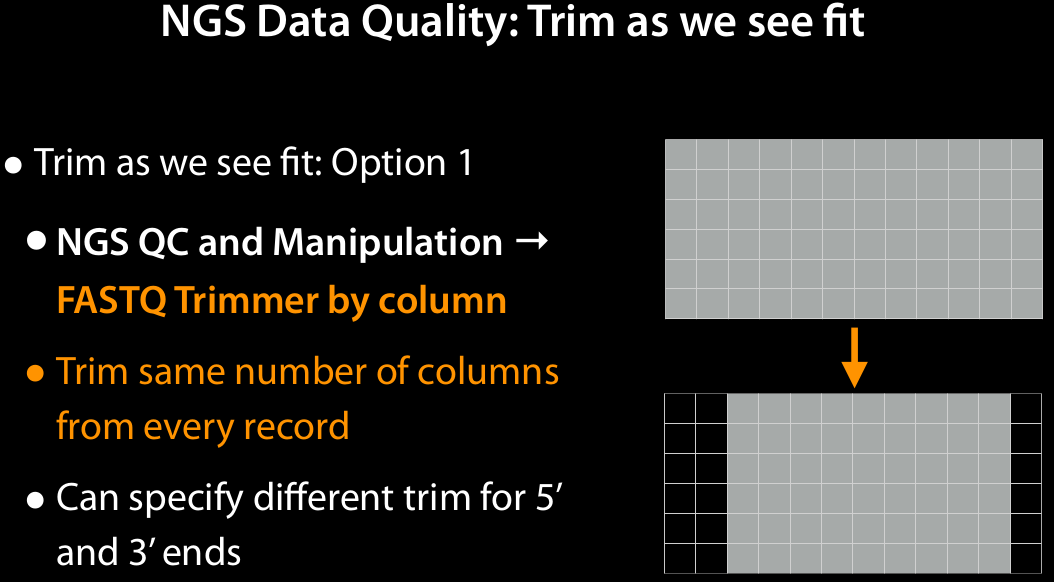
\includegraphics[width=\textwidth]{c2.genomics/supp.trim.01.png}
  \end{figure}
\end{frame}

\begin{frame}
  \frametitle{补遗 | 预处理 | Trim}
  \begin{figure}
    \centering
    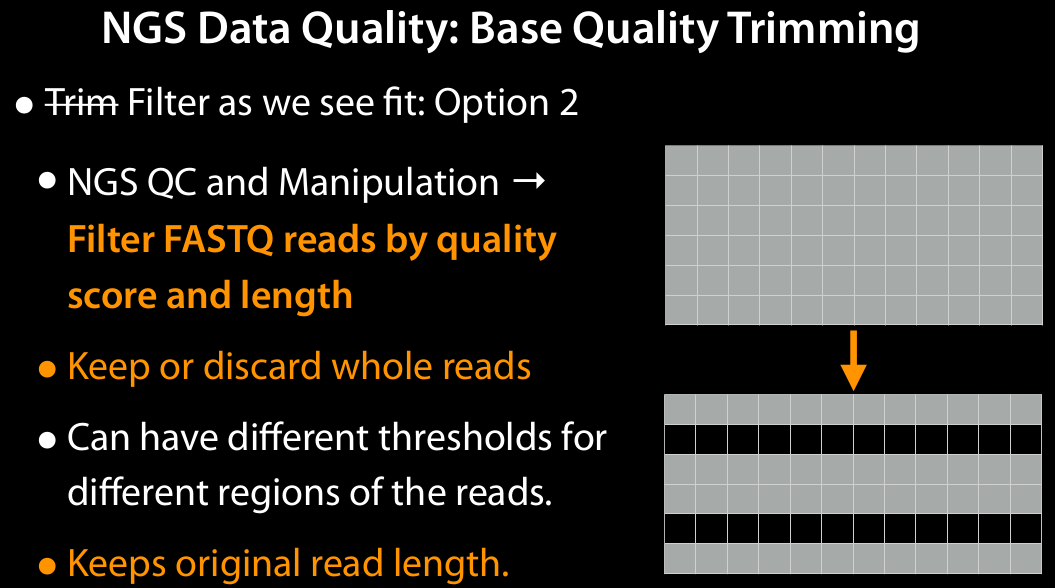
\includegraphics[width=\textwidth]{c2.genomics/supp.trim.02.png}
  \end{figure}
\end{frame}

\begin{frame}
  \frametitle{补遗 | 预处理 | Trim}
  \begin{figure}
    \centering
    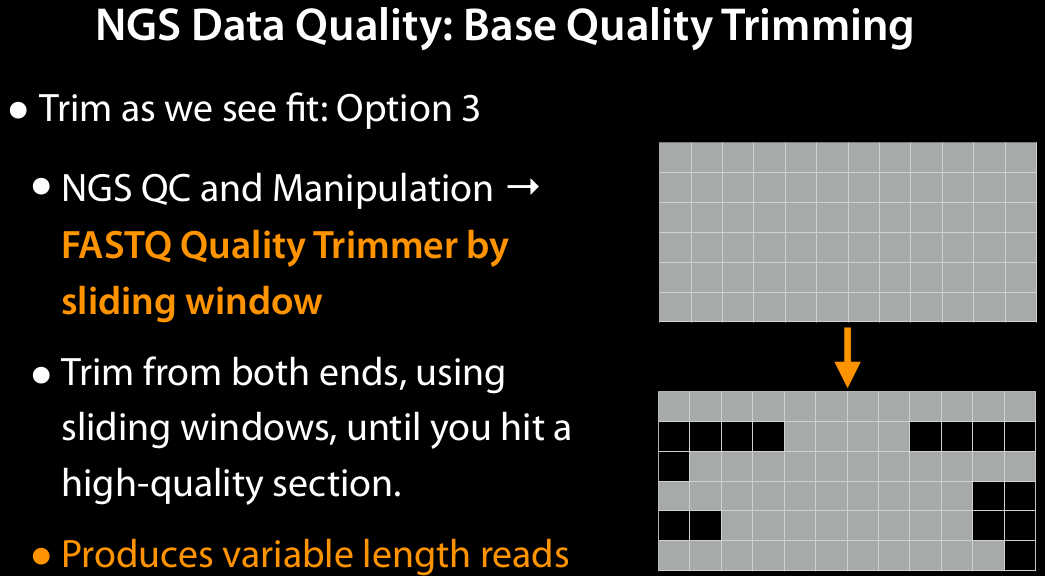
\includegraphics[width=\textwidth]{c2.genomics/supp.trim.03.png}
  \end{figure}
\end{frame}

\begin{frame}
  \frametitle{补遗 | 预处理 | Trim}
  \begin{figure}
    \centering
    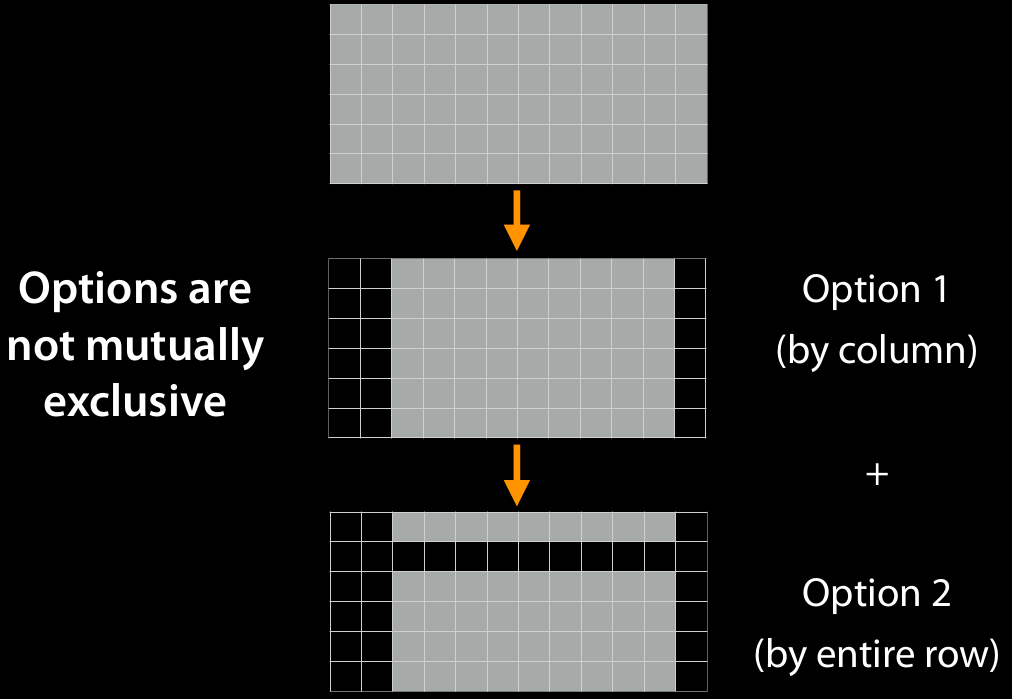
\includegraphics[width=0.9\textwidth]{c2.genomics/supp.trim.04.png}
  \end{figure}
\end{frame}

\begin{frame}
  \frametitle{补遗 | 预处理 | Trim}
  \begin{figure}
    \centering
    
\includegraphics[width=\textwidth]{c2.genomics/supp.trim.05.png}
  \end{figure}
\end{frame}

\subsection{比对后}
\begin{frame}
  \frametitle{补遗 | 比对 | Removal of PCR duplicates}
  \begin{figure}
    \centering
    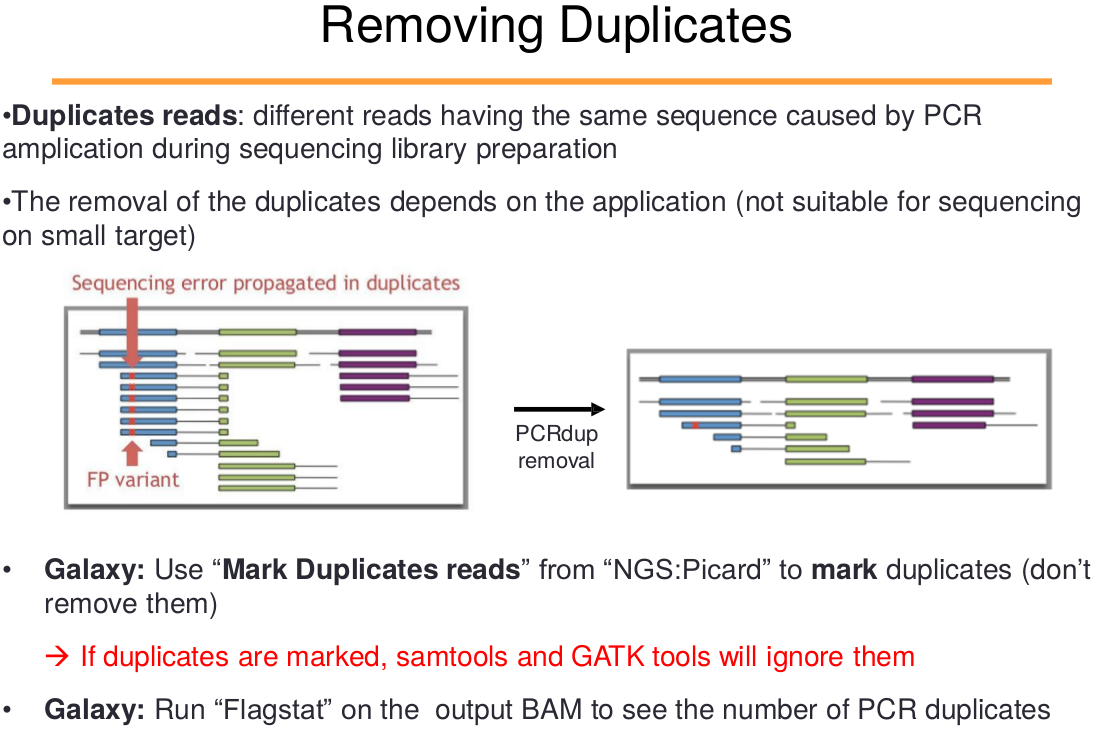
\includegraphics[width=0.9\textwidth]{c2.genomics/supp.dup.01.png}
  \end{figure}
\end{frame}

\begin{frame}
  \frametitle{补遗 | 比对 | Indel Realignment}
  \begin{figure}
    \centering
    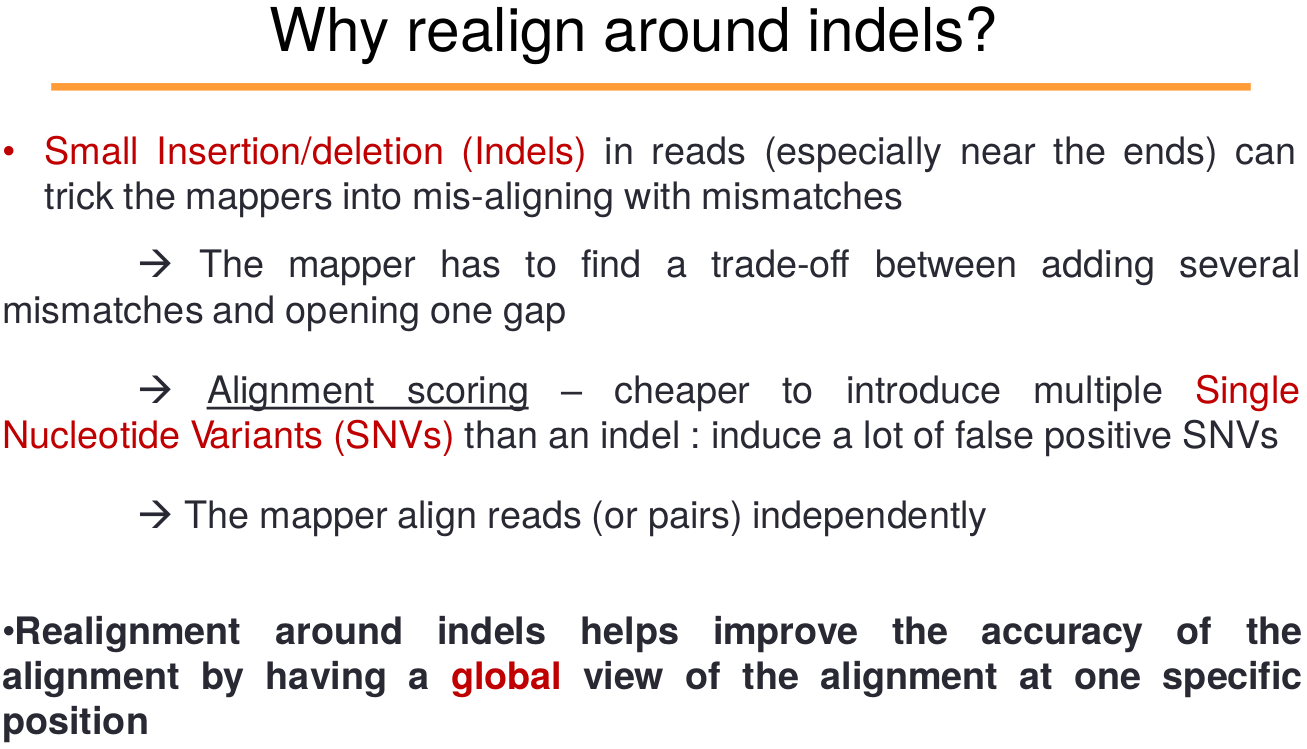
\includegraphics[width=\textwidth]{c2.genomics/supp.realign.01.png}
  \end{figure}
\end{frame}

\begin{frame}
  \frametitle{补遗 | 比对 | Indel Realignment}
  \begin{figure}
    \centering
    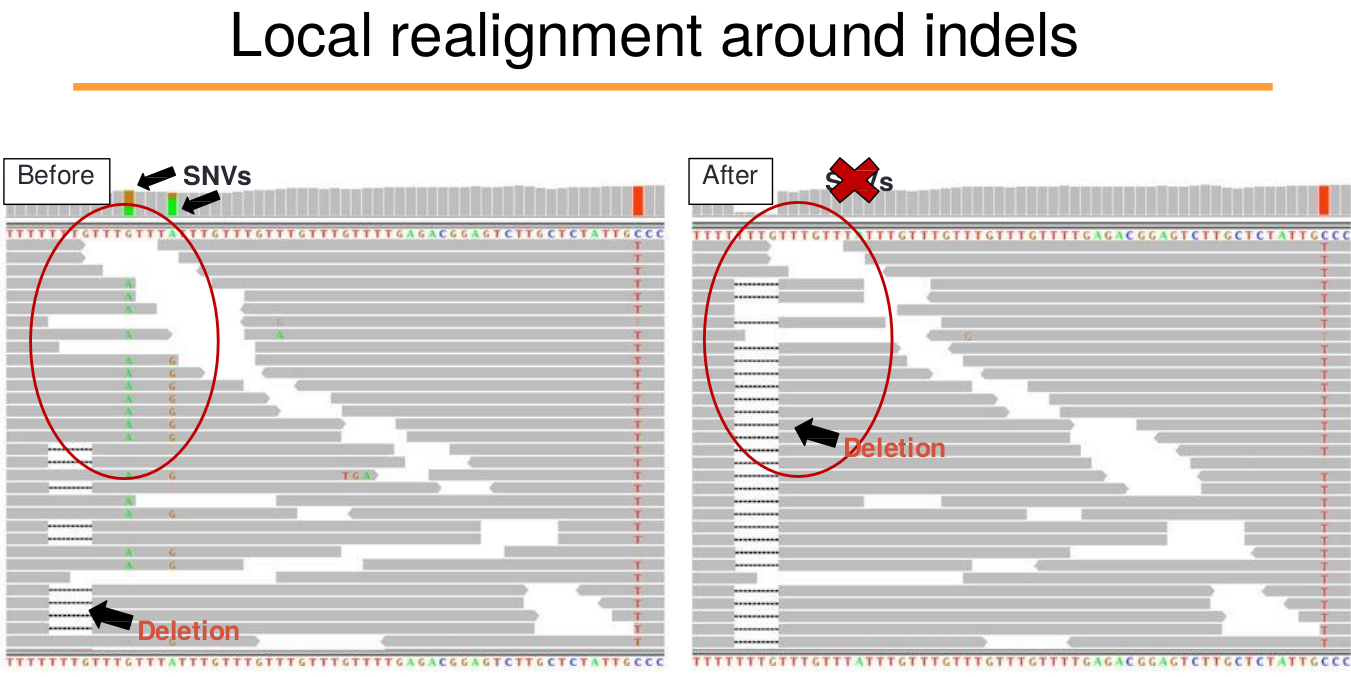
\includegraphics[width=\textwidth]{c2.genomics/supp.realign.02.png}
  \end{figure}
\end{frame}

\begin{frame}
  \frametitle{补遗 | 比对 | Indel Realignment}
  \begin{figure}
    \centering
    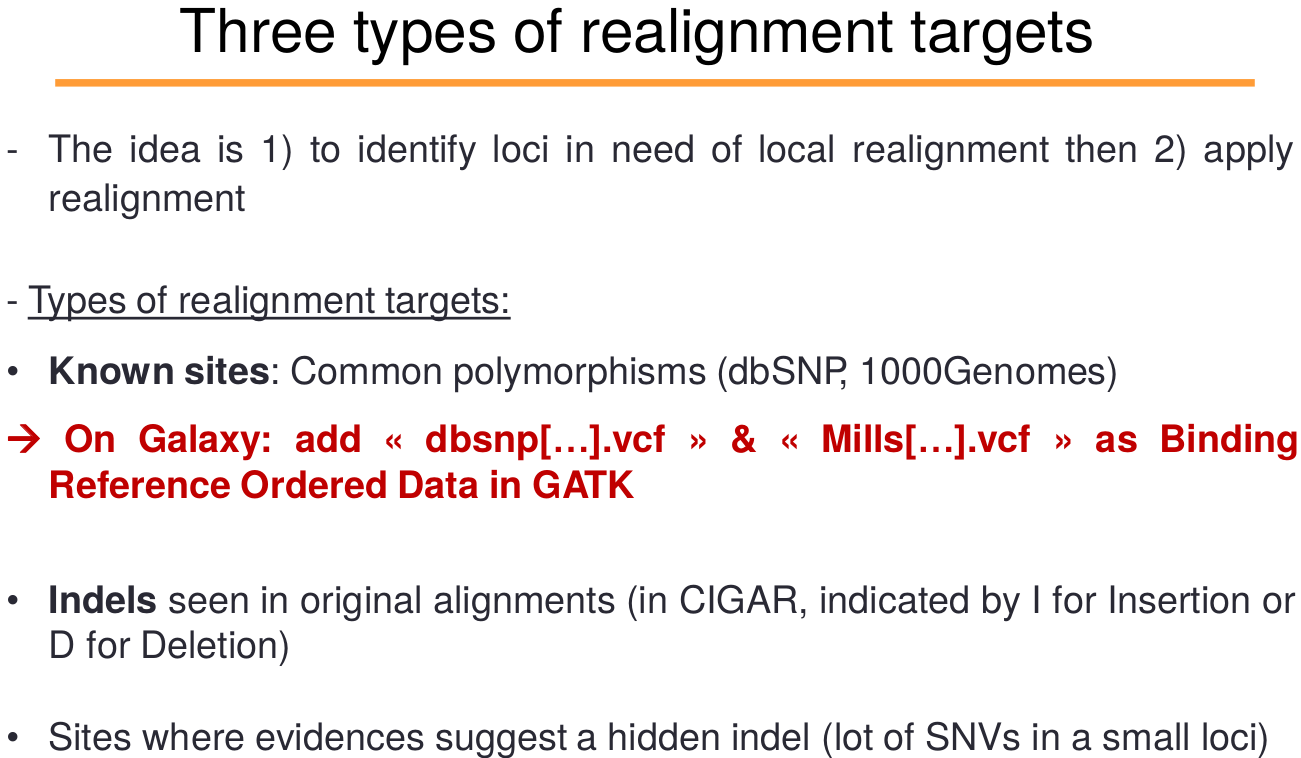
\includegraphics[width=\textwidth]{c2.genomics/supp.realign.03.png}
  \end{figure}
\end{frame}

\begin{frame}
  \frametitle{补遗 | 比对 | Indel Realignment}
  \begin{figure}
    \centering
    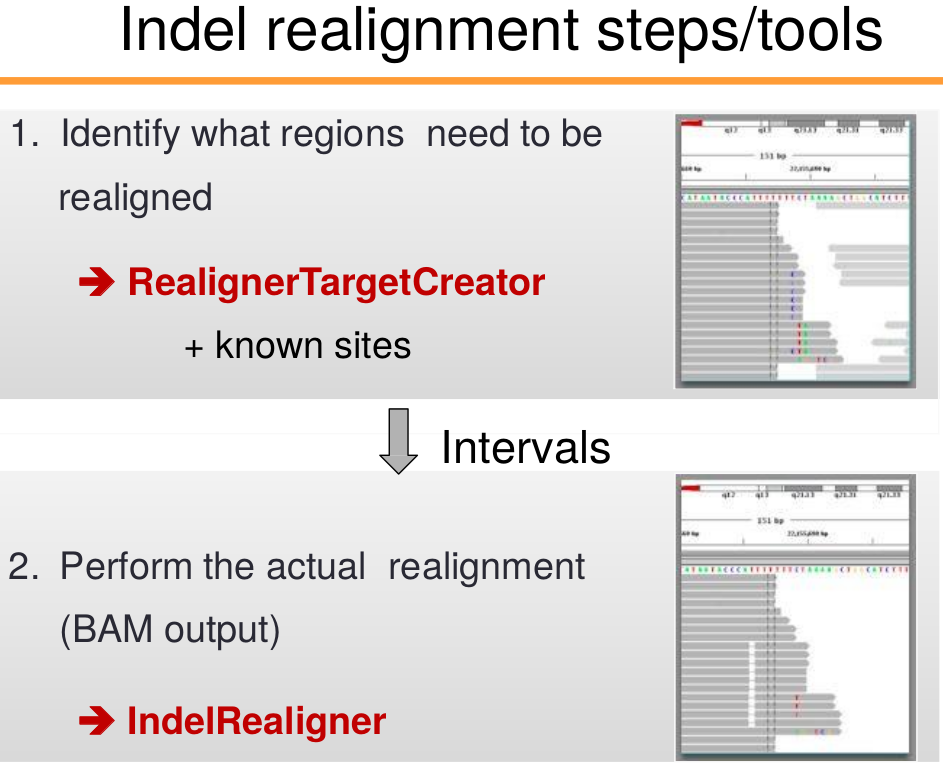
\includegraphics[width=0.8\textwidth]{c2.genomics/supp.realign.04.png}
  \end{figure}
\end{frame}

\begin{frame}
  \frametitle{补遗 | 比对 | Base quality recalibration}
  \begin{figure}
    \centering
    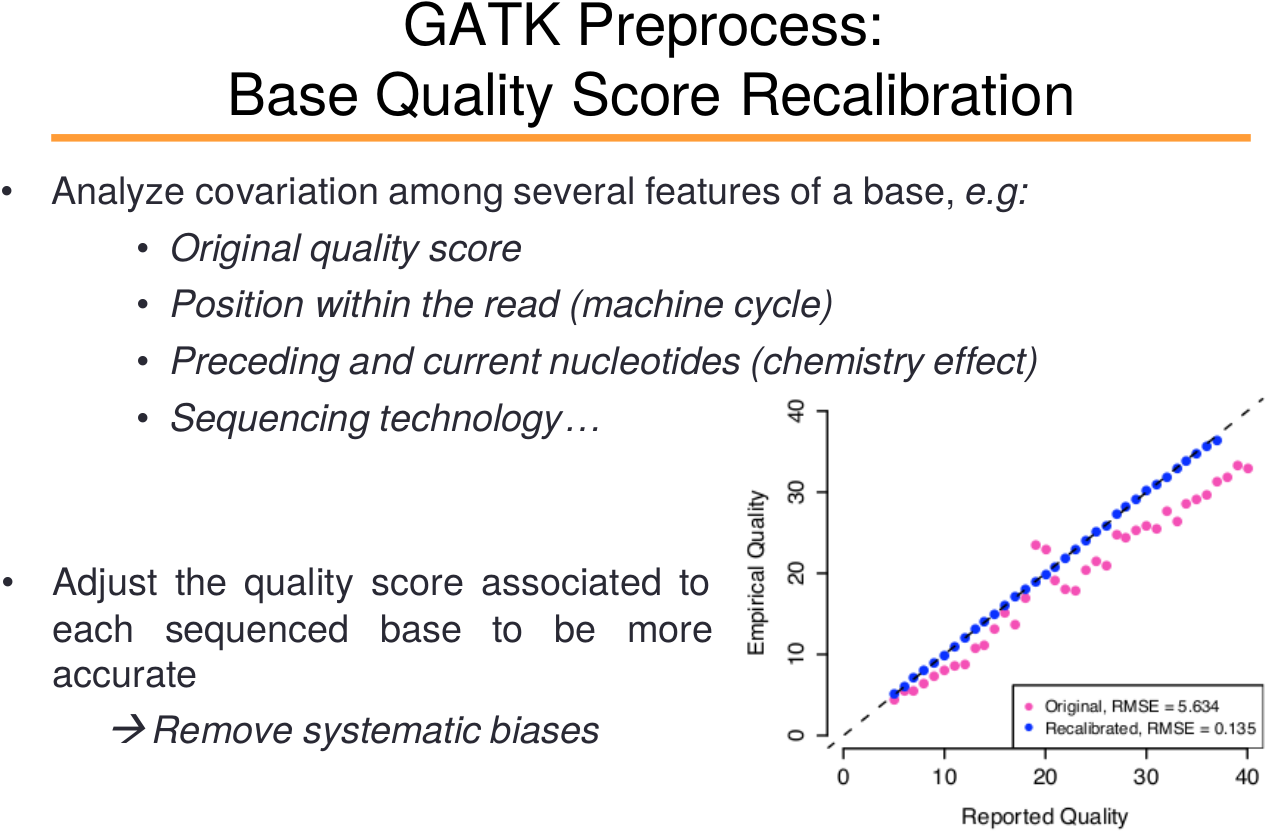
\includegraphics[width=\textwidth]{c2.genomics/supp.recal.01.png}
  \end{figure}
\end{frame}

\begin{frame}
  \frametitle{补遗 | 比对 | Base quality recalibration}
  \begin{figure}
    \centering
    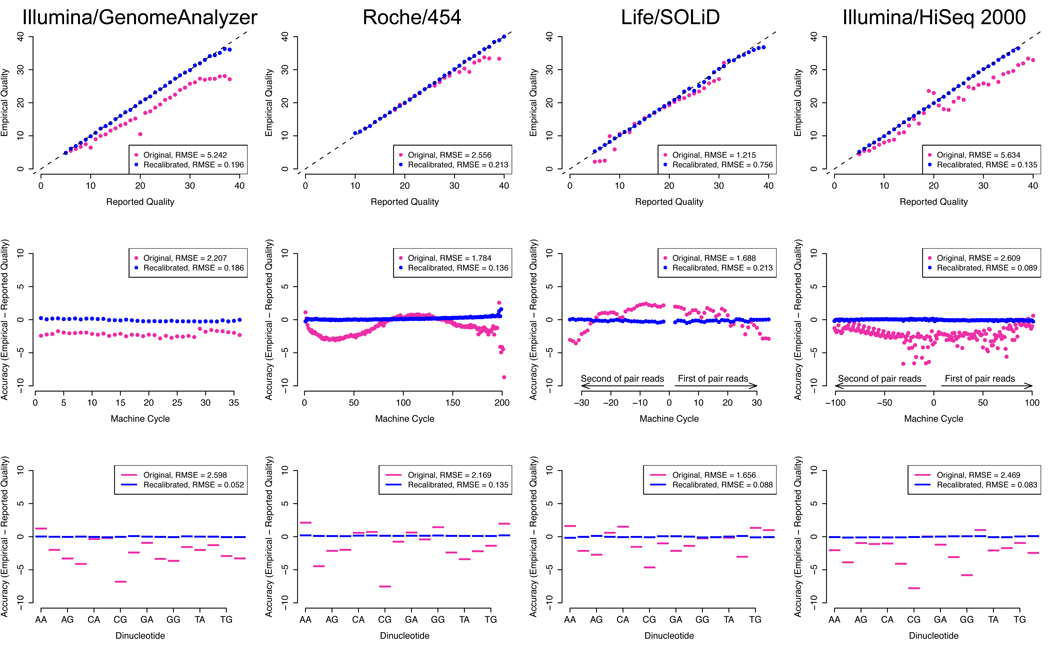
\includegraphics[width=\textwidth]{c2.genomics/supp.recal.02.jpg}
  \end{figure}
\end{frame}

\begin{frame}
  \frametitle{补遗 | 比对 | Base quality recalibration}
  \begin{figure}
    \centering
    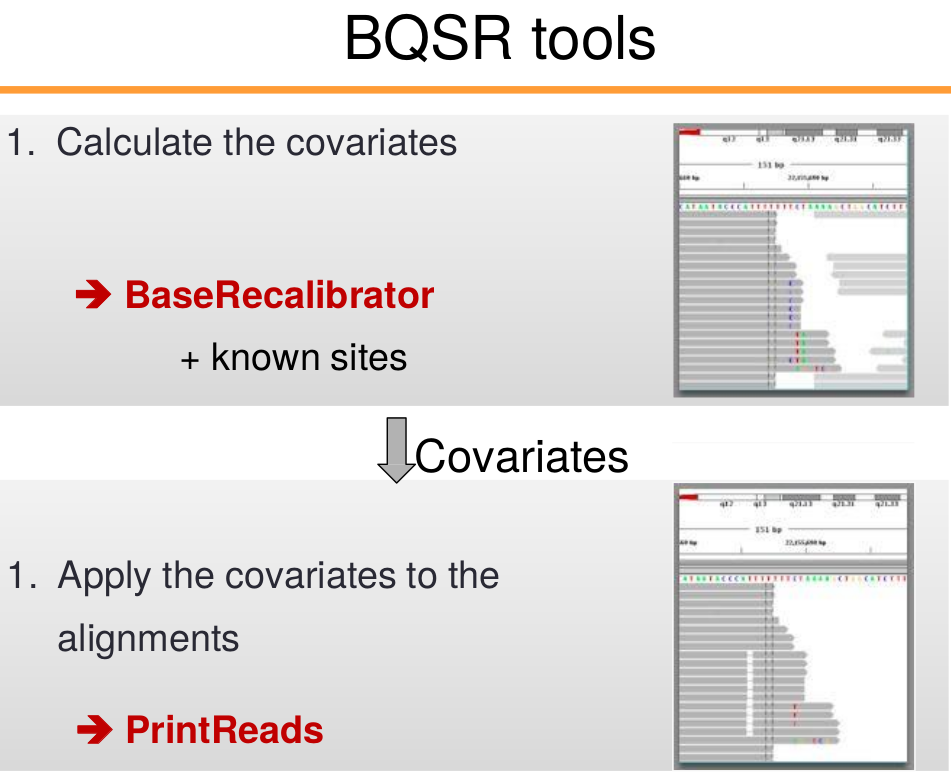
\includegraphics[width=0.8\textwidth]{c2.genomics/supp.recal.03.png}
  \end{figure}
\end{frame}

\subsection{实验设计}
\begin{frame}
  \frametitle{补遗 | 设计 | Replicates}
  \begin{figure}
    \centering
    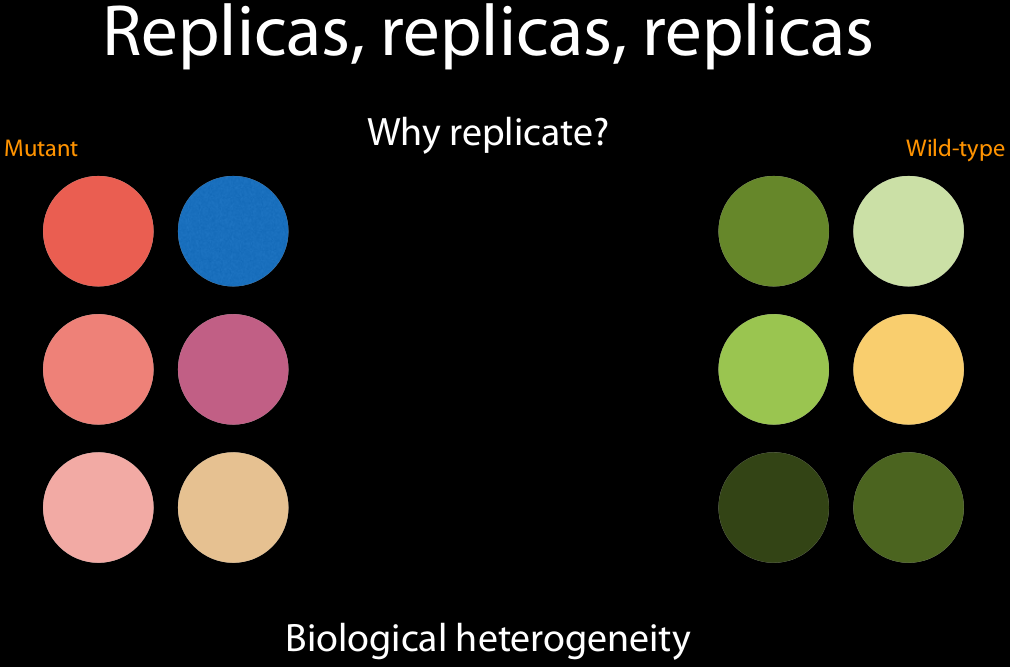
\includegraphics[width=\textwidth]{c2.genomics/supp.rep.01.png}
  \end{figure}
\end{frame}

\begin{frame}
  \frametitle{补遗 | 设计 | Replicates}
  \begin{figure}
    \centering
    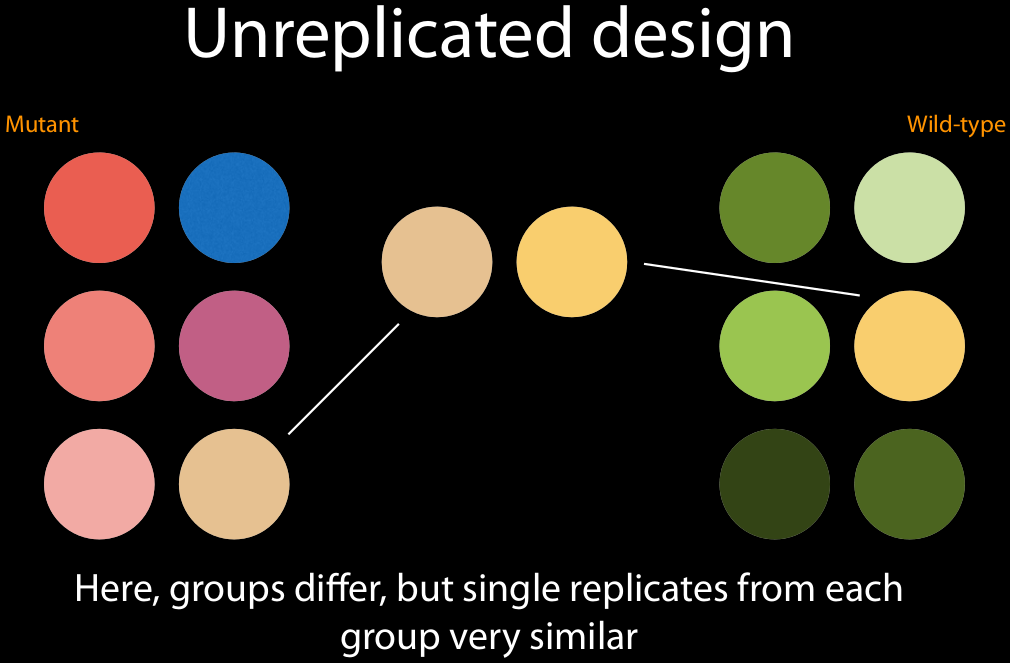
\includegraphics[width=\textwidth]{c2.genomics/supp.rep.02.png}
  \end{figure}
\end{frame}

\begin{frame}
  \frametitle{补遗 | 设计 | Replicates}
  \begin{figure}
    \centering
    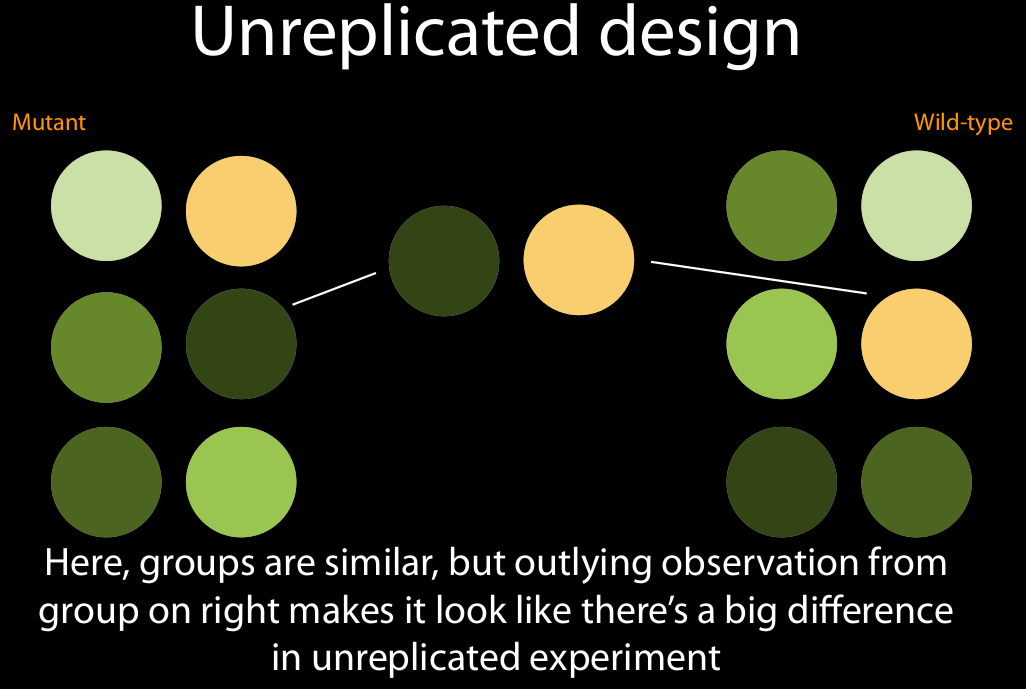
\includegraphics[width=\textwidth]{c2.genomics/supp.rep.03.png}
  \end{figure}
\end{frame}

\begin{frame}
  \frametitle{补遗 | 设计 | Replicates}
  \begin{figure}
    \centering
    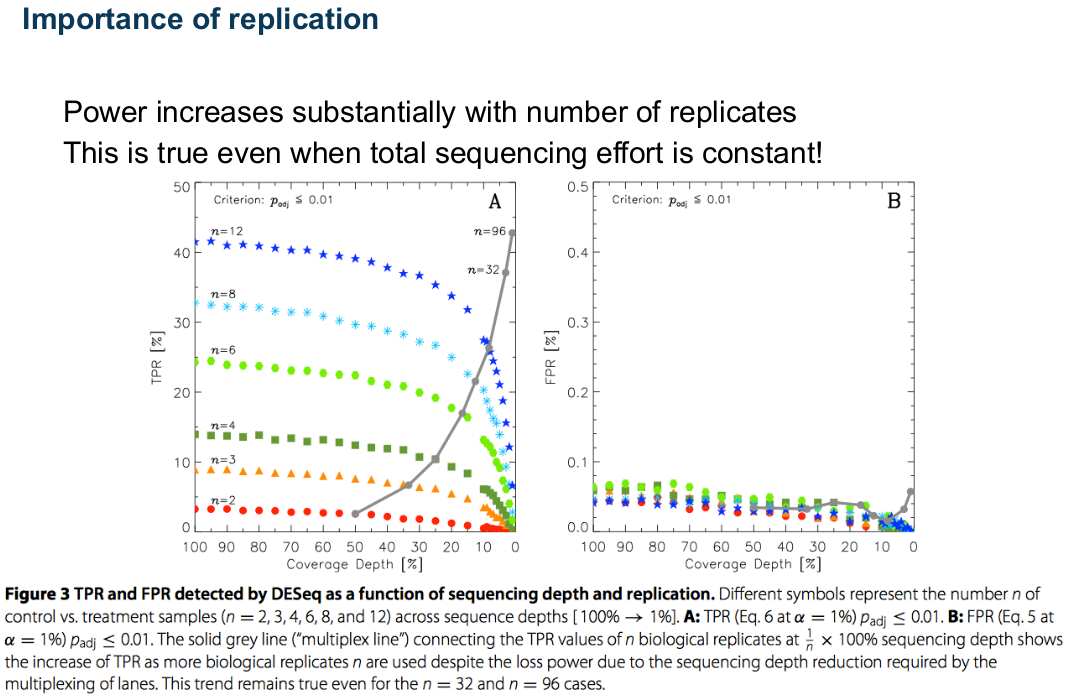
\includegraphics[width=\textwidth]{c2.genomics/supp.rep.04.png}
  \end{figure}
\end{frame}

\begin{frame}
  \frametitle{补遗 | 设计 | Replicates}
  \begin{figure}
    \centering
    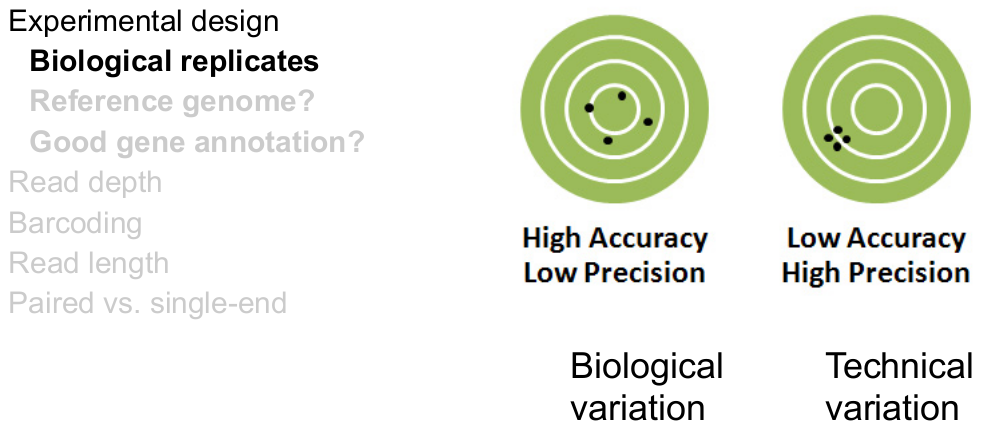
\includegraphics[width=\textwidth]{c2.genomics/supp.rep.05.png}
  \end{figure}
\end{frame}

\begin{frame}
  \frametitle{补遗 | 设计 | Replicates}
  \begin{figure}
    \centering
    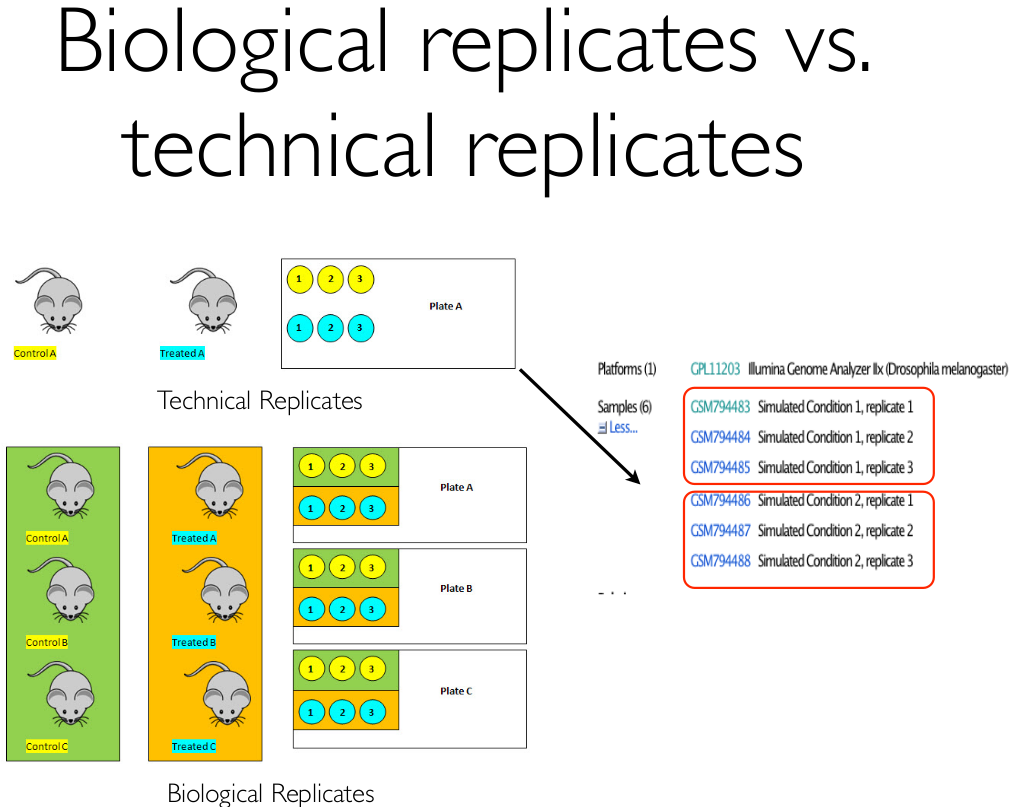
\includegraphics[width=0.8\textwidth]{c2.genomics/supp.rep.06.png}
  \end{figure}
\end{frame}

\begin{frame}
  \frametitle{补遗 | 设计 | Read depth}
  \begin{figure}
    \centering
    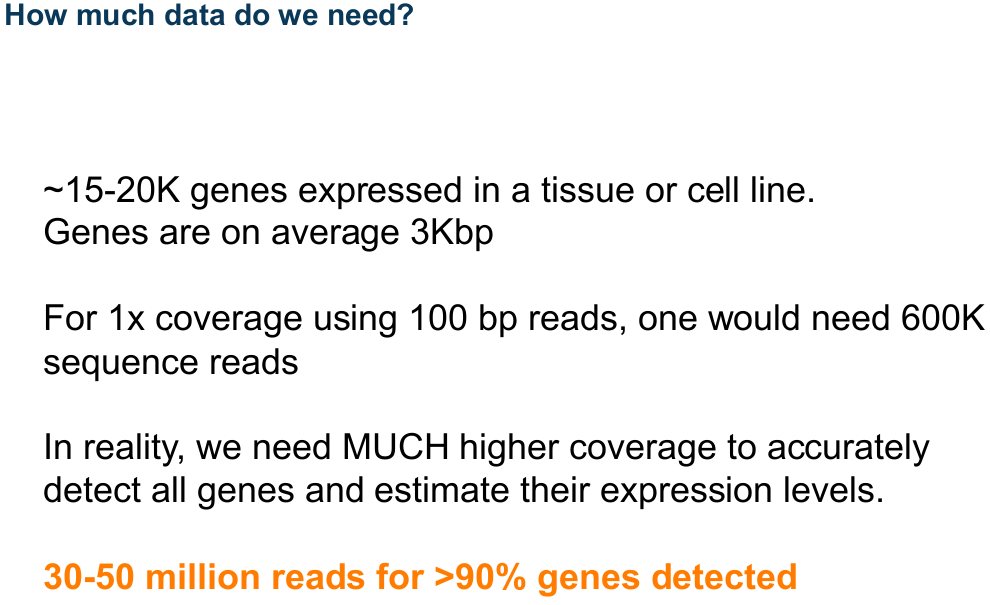
\includegraphics[width=\textwidth]{c2.genomics/supp.depth.01.png}
  \end{figure}
\end{frame}

\begin{frame}
  \frametitle{补遗 | 设计 | Read depth}
  \begin{figure}
    \centering
    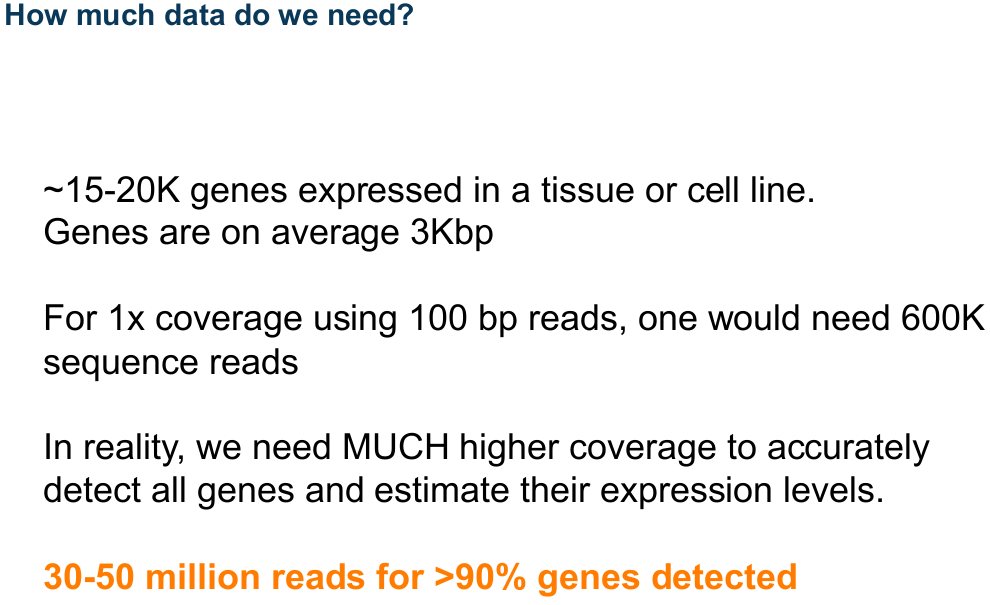
\includegraphics[width=\textwidth]{c2.genomics/supp.depth.01.png}
  \end{figure}
\end{frame}

\begin{frame}
  \frametitle{补遗 | 设计 | Read length}
  \begin{figure}
    \centering
    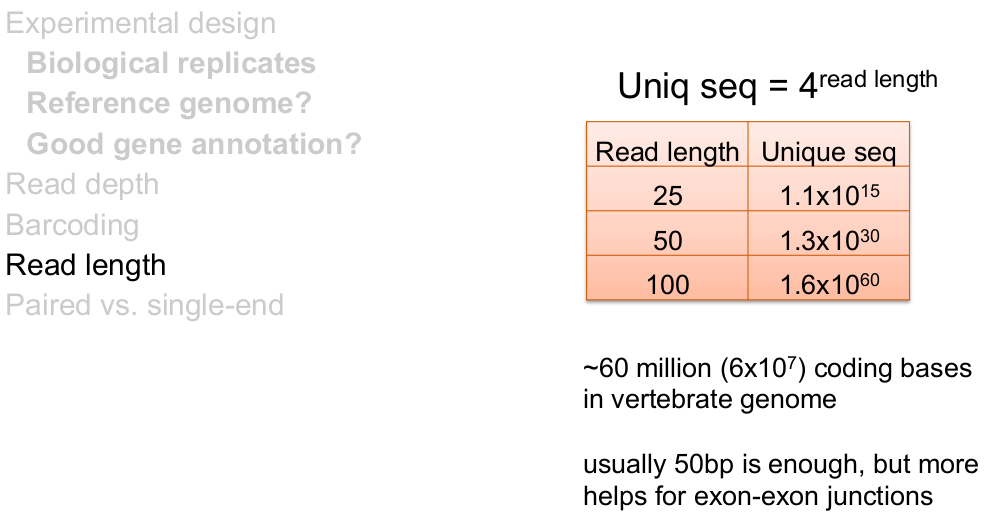
\includegraphics[width=\textwidth]{c2.genomics/supp.length.01.png}
  \end{figure}
\end{frame}

\begin{frame}
  \frametitle{补遗 | 设计 | Barcode}
  \begin{figure}
    \centering
    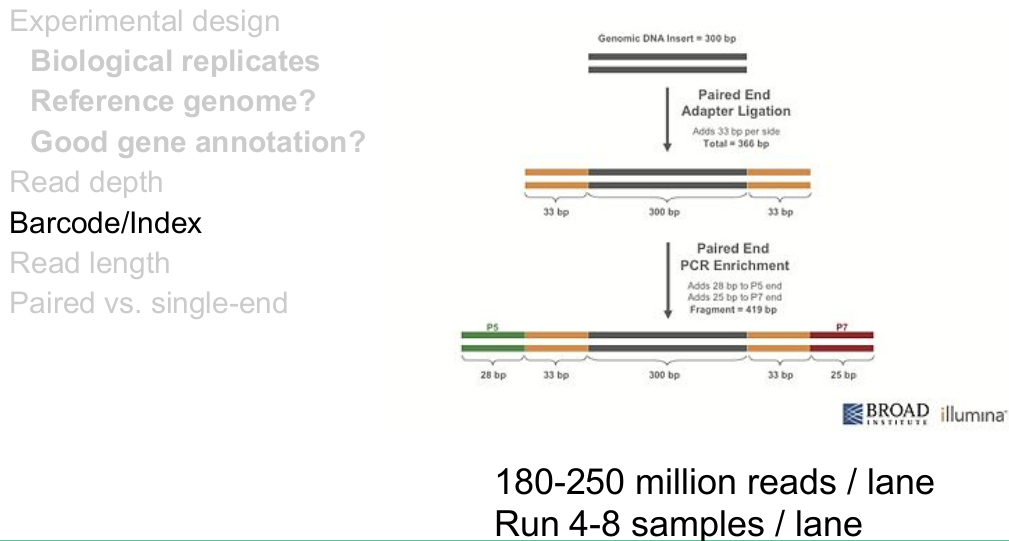
\includegraphics[width=\textwidth]{c2.genomics/supp.barcode.01.png}
  \end{figure}
\end{frame}

\begin{frame}
  \frametitle{补遗 | 设计 | \textcolor{red}{KEY}}
  \begin{figure}
    \centering
    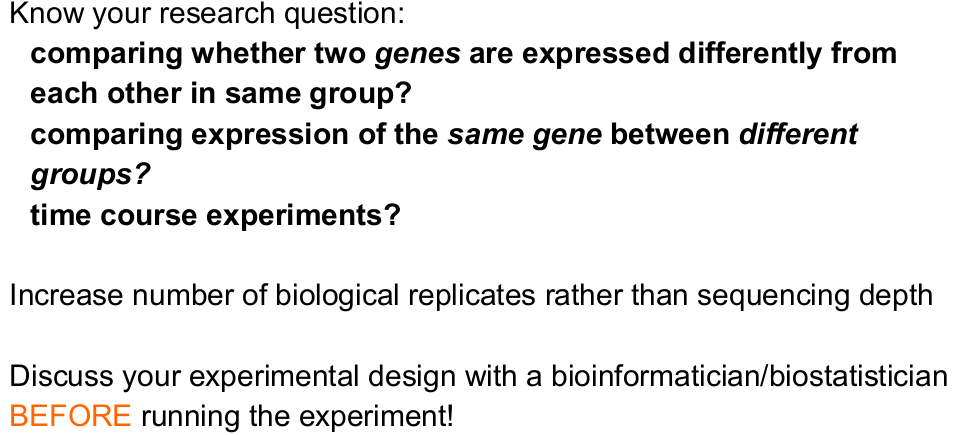
\includegraphics[width=\textwidth]{c2.genomics/supp.key.01.png}
  \end{figure}
\end{frame}

